\documentclass[10pt, a4paper]{article} % 设置字体大小和纸张类型
\usepackage{fontspec}
\setmainfont{Times New Roman}

\usepackage{booktabs} % 支持更专业的表格线条
\usepackage{ctex}
\usepackage{caption} % 插图和表格的标题格式
\usepackage{amsmath, amsfonts, amssymb} % 数学公式支持
\usepackage{graphicx} % 插入图片
\usepackage{hyperref} % 超链接支持
\usepackage{geometry}
\usepackage{titlesec}
\usepackage{fmtcount} % 用于数字到中文的转换
\usepackage{enumitem} % 加载 enumitem 宏包
\usepackage{multirow} % 支持多行单元格
\usepackage{diagbox}
\usepackage{makecell} % 支持单元格内换行
\usepackage{tikz}
\usepackage{booktabs} % 支持更专业的表格线条
\usepackage{multirow} % 支持多行单元格
\usepackage{makecell}
\usepackage{unicode-math}
\setmathfont{Latin Modern Math}
\geometry{a4paper, margin=1.5cm} % 设置页边距

\renewcommand{\thesection}{\chinese{section}、}
\renewcommand{\thesubsection}{\arabic{subsection}.}

\begin{document}

\begin{titlepage}
    \newgeometry{left=0cm, right=0cm, top=0cm, bottom=0cm}
    \centering
    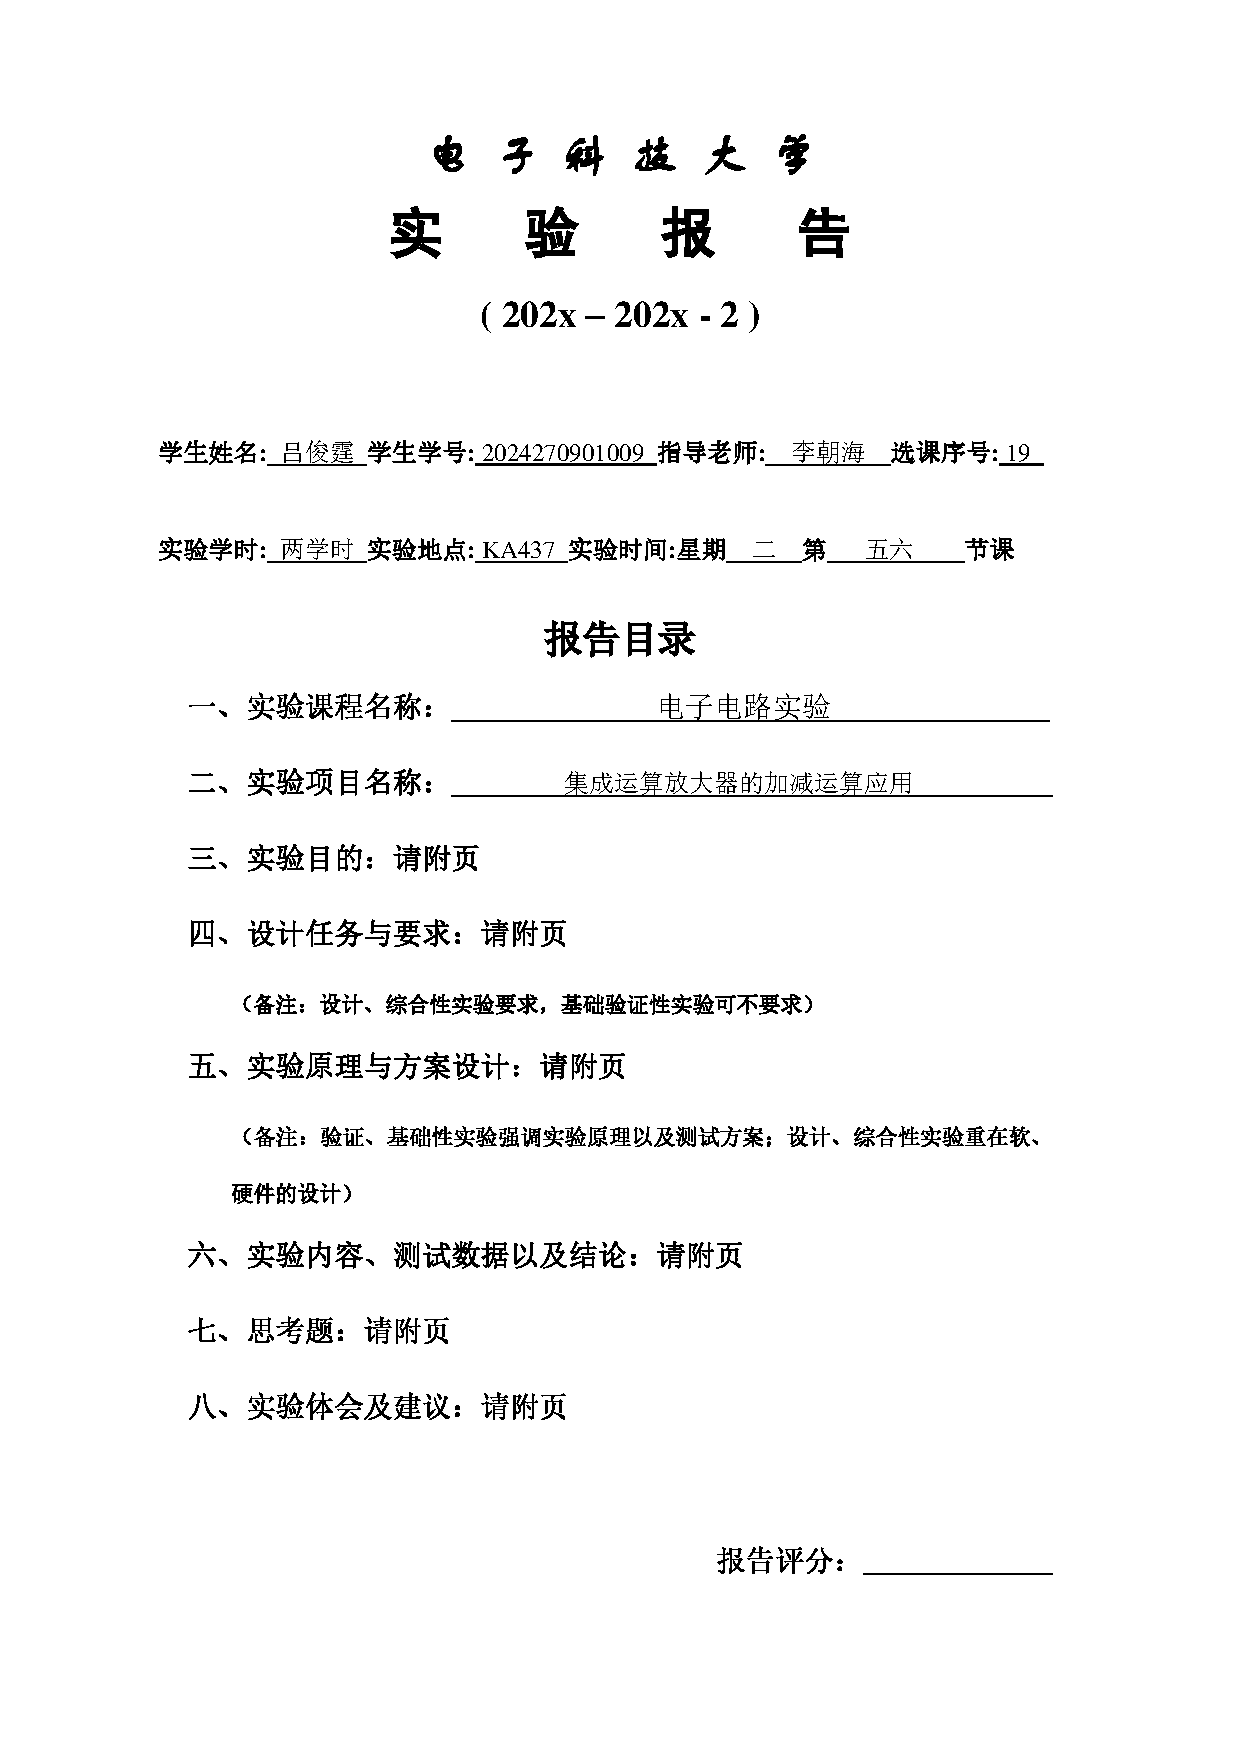
\includegraphics[page=1, width=0.9\textwidth, keepaspectratio]{image/实验报告撰写封面.pdf}
    \restoregeometry
\end{titlepage}

\setcounter{section}{2}

\end{document}